\documentclass[conference]{IEEEtran}
\usepackage[style=ieee, backend=biber]{biblatex}
\usepackage[T1]{fontenc}
\usepackage{array}
\usepackage{url}
\usepackage{eso-pic}

\ifCLASSINFOpdf
	\usepackage[pdftex]{graphicx}
	\graphicspath{{img/}}
	\DeclareGraphicsExtensions{.pdf,.jpg,.png, .eps}
\else
	\usepackage[dvips]{graphicx}
 	\graphicspath{{img/}}
	\DeclareGraphicsExtensions{.pdf,.jpg,.png, .eps}
\fi

\hyphenation{op-tical net-works semi-conduc-tor}

\bibliography{paper.bib}

\begin{document}

\IEEEoverridecommandlockouts 
\IEEEpubid{\begin{minipage}{\textwidth}\ \\[30pt] \\\textbf{IEEE/ACM ASONAM 2016, August 18-21, 2016, San Francisco, CA, USA\\ 978-1-5090-2846-7/16/\$31.00\copyright2016 IEEE} \end{minipage}} 

\AddToShipoutPictureBG*{ 
\AtPageUpperLeft{ 
\setlength\unitlength{1in} 
\hspace*{\dimexpr0.5\paperwidth\relax}
\makebox(0,-0.75)[c]{\textbf{2016 IEEE/ACM International Conference on Advances in Social Networks Analysis and Mining (ASONAM)}}}} 

\title{Mimicry in Online Conversations: An Exploratory Study of Linguistic Analysis Techniques}
\author{\IEEEauthorblockN{Tom Carrick, Awais Rashid, Paul J Taylor}
\IEEEauthorblockA{Security Lancaster / CREST\\
Lancaster University\\
Lancaster, United Kingdom\\
Email: \{t.carrick, a.rashid, p.j.taylor\} @lancaster.ac.uk}}

\maketitle

\begin{abstract}
A number of computational techniques have been proposed that aim to detect mimicry in online conversations. In this paper, we investigate how well these reflect the prevailing cognitive science model, i.e. the Interactive Alignment Model. We evaluate Local Linguistic Alignment, word vectors, and Language Style Matching and show that these measures tend to show the features we expect to see in the IAM, but significantly fall short of the work of human classifiers on the same data set. This reflects the need for substantial additional research on computational techniques to detect mimicry in online conversations. We suggest further work needed to measure these techniques and others more accurately.

\end{abstract}


\IEEEpeerreviewmaketitle


\section{Introduction}

When interacting with others, humans show a tendency to mimic one another's behavior, including speech \cite{levelt1982surface, bock1986syntactic, bock1989closed, garrod1987saying}, physical actions \cite{bernieri1988coordinated} and written text \cite{danescu2011chameleons, scissors2008linguistic}. Existing research has shown that people who mimic each other's language have more successful outcomes in joint tasks \cite{richardson2014language}, and that decreasing mimicry can be an indicator of deception \cite{taylor2013detecting}. Hence, detection of mimicry can be a valuable indicator in dyadic conversations as well as group dynamics in collaborative settings \cite{scissors2009cmc}. Potential applications include promoting cooperation, detecting malintent, and identifying leaders.

There are a number of measures designed to capture mimicry in text, and some efforts have been made to compare and trial some of these techniques \cite{xu2015evaluation}. However, few techniques are grounded in what cognitive science knows about how mimicry works within humans. That is to say, few of the existing techniques are designed to measure the linguistic components of verbal mimicry as specified by contemporary models from cognitive science.

This paper addresses this limitation by contrasting how well existing linguistic analysis techniques work to detect mimicry in relation to a prominent model of human interpersonal mimicry, the Interactive Alignment Model. Further, we consider some existing techniques that have not previously been used to detect mimicry and discuss their viability. The novel contributions of this paper are as follows:
\begin{itemize}
	\item We compare two existing mimicry detection techniques and how they map to the Interactive Alignment Model, Local Linguistic Alignment \cite{wang2014linguistic} and Language Style Matching \cite{ireland2010language}.
	\item  We evaluate and discuss the feasibility of using word vectors \cite{mikolov2013efficient} to measure semantic mimicry.
	\item We find how one measure, Language Style Matching \cite{ireland2010language}, that does not appear to fit into the model, may nevertheless have a place in the model.
\end{itemize}

The rest of this paper is structured as follows. In Section II, we briefly introduce the Interactive Alignment Model. Section III provides a brief introduction to each measure tested in the paper, and defines the layer of the IAM (if any) in which the measure appears to reside. Section IV describes the data set used in our analysis. Section V presents the results of our analysis and highlights how current techniques fit into the IAM in practice. Finally, Section VI concludes the paper and identifies directions for future work.

\section{The Interactive Alignment Model}
In order to achieve conversation, two or more interactants must work together to establish a joint understanding of what they are talking about. The Interactive Alignment Model (IAM) \cite{pickering2004toward, garrod2004conversation}, shown in Fig. \ref{iam} is an attempt to model such alignment as it occurs over time in conversations. It consists of six layers, which with the exception of the top layer, the situation model, are all representations of different linguistic levels at the same time, as understood by each speaker within an interaction. In basic terms, these levels are:

\begin{enumerate}
	\item The situation model --- a representation of the situation being discussed
	\item The semantic representation --- the meaning of the utterance in terms of what it stands to convey.
	\item The syntactic representation --- the sentence structure
	\item The lexical representation --- the choice of words used
	\item The phonological representation --- the abstract representation of word sounds
	\item The phonetic representation --- the sounds of an utterance
\end{enumerate}

The theory states that alignment is automatic and that conversation partners will 'interactively align' their speech  towards each other at every level of the model. The observable behavior of such alignment is greater mimicry at each layer.

The IAM also postulates how such alignment emerges over time. It suggests that alignment 'percolates' between layers such that increased alignment in one layer will lead to increased alignment in other layers. For example, tightening the semantic representation will naturally restrict the number of words and syntactic structures that can be used to convey that meaning. Similarly, particular word choices may shape the kinds of semantic representations that become prominent. In short, alignment at one level enables a listener to fill in the gaps and appropriately mimic at another level.

The phonological and phonetic representations are not discussed in this paper as they relate purely to the sound of speech, representations that do not exist in the written text of online conversations. Further, the situation model is not included as there are currently no measures that can be used for finding alignment at the situational level.

\begin{figure*}
\caption{The interactive alignment model}
\label{iam}
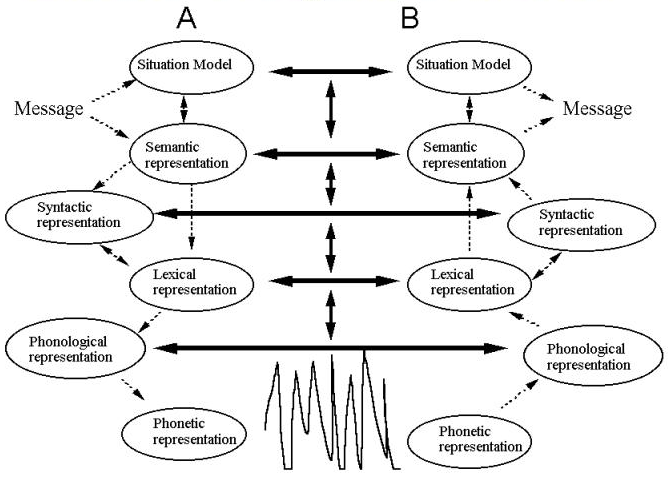
\includegraphics[width=\textwidth]{iam}
\end{figure*}


\section{Analysis Techniques}

There are many techniques for finding mimicry, but few of them specifically target any layer of the IAM. We chose one measure for each layer, as well as Language Style Matching to have a technique that could fit into the lexical layer, or could be seen to work outside of the IAM.

Techniques were chosen mostly to try to fit into a layer of the IAM. Simplicity of implementation and access to source implementations was also a factor, and modern techniques were favoured over older ones.


\subsection{Local Linguistic Alignment}
Local Linguistic Alignment (LLA) is a simple, dual purpose method that can work at both the lexical and syntactic layers \cite{wang2014linguistic, xu2015evaluation}. LLA was chosen specifically as it was the only measure the authors could find where it is explicitly stated to work at the lexical and syntactic layers.

Lexical Indiscriminate Local Linguistic Alignment (LILLA) works at the lexical layer. It gives the probability that a word from the prime document will appear at a particular position in the target  document. It is defined as:

\[LILLA(target, prime) = \frac{p(target|prime)}{p(target)}\]

Syntactic Indiscriminate Local Linguistic Alignemnt (SILLA) works at the syntactic layer. It works in exactly the same way as LILLA, but instead of comparing words, each sentence is annotated with a phrase structure tree, and LLA is run on these instead. As such, it measures the probability of a phrase structure subtree in the prime document appearing occurring at a given position in the target document.


\subsection{Word Vectors}
Word2vec \cite{mikolov2013efficient, mikolov2013distributed} is a machine learning technique that, given a word, tries to predict the two adjacent words. Each word is then mapped to vector space and can be directly compared. The closer the two word vectors to each other, the more semantically related they are.

While word vectors have not been used to measure mimicry before, we posit that it may give good results for finding mimicry as it is used for finding semantic similarity in text, we would expect it to also find semantic mimicry.


\subsection{Language Style Matching}
Language Style Matching (LSM) \cite{ireland2010language, ireland2011language} is a measure that counts the usage of function words by an interlocutor. For each class of function word (e.g., determiners, pronouns, adpositions), the number of words is  calculated as a percentage of the total document, which is the score for each class. Scores are calculated between the dyad using a weighted difference, shown below, and these scores averaged to produce a single LSM score for that dyad.

\[ LSM_{class} = 1 - [(|class_1 - class_2|)] / (class_1 + class_2 + .0001) \]


\section{Method}
The data set consists of 103 dyadic conversations taken from Twitter. Tweets were found via Twitter's  search API, using English language and being a reply as criteria. We then work up the chain of tweets  until we hit the end, or a third interlocutor is found, at which point the conversation is cut off and  kept, as long as there are no fewer than 10 tweets in the conversation. 200 tweets were found using  this method. Of these, 62 were removed as they were not true conversations (either monologues or  collaborative fiction writing/roleplay). 18 conversations were removed as they had significant amounts  of non-English text. 17 conversations involved bots and were also removed.

The data was processed as follows:
\begin{itemize}
	\item Screen names at the start of the message were removed. These are just the names of the 
		  interlocutors and only add noise.
	\item All URLs were replaced with the string '[URL]'.
	\item HTML entities such as \&amp; were converted to plain text (\&).
	\item Any adjacent messages by the same author were merged together such that each message always
	      alternates between the two interlocutors.
\end{itemize}

Twitter was chosen as it is relatively easy to extract data from, and the short utterance and conversation length make it more reasonable for humans to classify, as with longer texts they may find more difficulty in keeping less recent utterances in mind while evaluating more recent ones. 

The data set is small, which is both an advantage as it is possible to classify the data manually and a disadvantage in that the sample size is smaller. We did not actively seek out mimicry by targeting our search as it was important to have conversations that would test negatively for mimicry as well as positively.

The data was classified by three researchers with backgrounds in mimicry independent of the authors of  this paper. Each  conversation was classified for lexical, syntactic and semantic mimicry on a three point scale  where 0 represents no mimicry, 1 represents low levels of mimicry at that layer, and 2 represents high  levels of mimicry. Classifications from each author were averaged together to give each conversation three scores between 0 and 2.

Each measure was then run against the data such that each message from author A is compared with each  message from author B that occurred before the original message. \footnote{Source code available at \url{https://github.com/knyghty/linguistic-analysis}.}


\section{Results and Disucssion}

\begin{table}[!t]
\caption{Correlations of Classifiers With Each Other}
\label{classifiers}
\centering
\renewcommand{\arraystretch}{1.2}
\begin{tabular}{l | c c | c c | c c}
Pair & \multicolumn{2}{|c|}{Lexical} & \multicolumn{2}{|c|}{Syntactic} & \multicolumn{2}{|c}{Semantic} \\
 & r & p & r & p & r & p \\
\hline
AB & 0.28 & 0.779 & 0.36 & < 0.001 & 0.19 & 0.058 \\
AC & 0.32 & 0.001 & 0.35 & < 0.001 & 0.12 & 0.220 \\
BC & -0.02 & 0.863 & 0.29 & 0.003 & 0.10 & 0.312
\end{tabular}
\end{table}

Table \ref{classifiers} shows the correlations between the scores of each pair of classifiers. In general, the human classifiers agreed with each other, but the agreement is fairly weak. They most strongly agreed on syntactic mimicry. Additionally there seemed to be more agreement on lexical mimicry than semantic, but p values are too high to make a definitive judgment.

\begin{table}[!t]
\caption{Correlations of Classifier Scores and Techniques}
\label{scores_techniques}
\centering
\renewcommand{\arraystretch}{1.2}
\begin{tabular}{l c c}
Layer, Technique & r & p \\
\hline
Lexical, LILLA & 0.27 & 0.005 \\
Syntactic, SILLA & 0.19 & 0.057 \\
Semantic, Word2vec & 0.13 & 0.178 \\
Lexical, LSM & 0.14 & 0.158 \\
Syntactic, LSM & 0.31 & 0.002 \\
Semantic, LSM & -0.13 & 0.202 \\
N/A (mean scores), LSM & 0.16 & 0.111
\end{tabular}
\end{table}

Table \ref{scores_techniques} shows the correlations between the mean scores from the human classifiers with the measure they should fall into.  Additionally means of all human classifier scores were used as a comparison with LSM, and LSM was compared with all other scores, to see where it best fits within the IAM. We see that scores from human classifiers show positive but weak correlation with the scores from their respective techniques. Additionally, LSM has a much better correlation with our syntactic scores than any other. Despite operating at the word level, LSM appears to be more of a syntactic measure than a lexical measure. This makes some sense when considering that choosing different function words may force a change of syntax.

\begin{table}[!t]
\caption{Correlations of Techniques}
\label{techniques}
\centering
\renewcommand{\arraystretch}{1.2}
\begin{tabular}{l c c}
Technique & r & p \\
\hline
LILLA, SILLA & 0.26 & 0.007 \\
LILLA, Word2vec & -0.30 & 0.005 \\
SILLA, Word2vec & -0.82 & < 0.001
\end{tabular}
\end{table}

Table \ref{techniques} shows the correlations of the computational methods with each other, to observe the IAM's prediction that increased levels of mimicry on one layer results in a higher probability of mimicry in other adjacent layers. The comparison of LILLA and SILLA is quite promising, however the strong negative correlations when word vectors are involved are both concerning and interesting, as this is the opposite of what we expect.

\begin{table}[!t]
\caption{Correlations of Human Classifications}
\label{classifications}
\centering
\renewcommand{\arraystretch}{1.2}
\begin{tabular}{l c c}
Layer & r & p \\
\hline
Lexical, Syntactic & 0.57 & < 0.001 \\
Lexical, Semantic & 0.33 & < 0.001 \\
Syntactic, Semantic & 0.28 & 0.005
\end{tabular}
\end{table}

Table \ref{classifications} shares the same idea, but compares the human classifiers' lexical, syntactic and semantic scores with each other. Here, the results are much closer to what we expect, with moderate positive correlations between all layers. The contrast with the word vector results from Table \ref{techniques} suggest that word vectors may not be a good solution for finding semantic mimicry, but doesn't explain the strong negative correlation between SILLA and Word2vec. The strong correlation between human classifiers' lexical and syntactic scores compared with the weaker correlation between LILLA and SILLA could suggest that humans are better suited for this task.

As results involving the semantic layer generally lead to lower levels of correlation, it could be argued that discerning semantic mimicry is a harder task than for the lexical and syntactic layers. However, it should be noted that there is still a weak to moderate positive correlation.

Even defining semantic mimicry was found to be a difficult task. It seems to make little sense to say that semantic mimicry is present where the same subject is discussed, as there are few situations where interlocutors will have a conversation about different things at the same time. It also makes little sense to define it as agreement with the other interaction partner, as agreement could be natural, rather than evidence of mimicry. Instead, we defined semantic mimicry as the people in the conversation communicating using similar concepts. This seems to be difficult for humans to analyse, especially from short twitter conversations, and could help to explain why computational methods also find this task difficult.


\section{Conclusion and Future Work}

We have presented some initial findings from our study into mimicry in online conversations. We have found that current computational methods are not especially good at finding mimicry in accordance with the Interactive Alignment Model, and that human experts currently seem to do a somewhat better job.

Our results further show support for the IAM's theory that mimicry in one layer increases the chance of mimicry in the other layers.

More research is needed, particularly in the methods used to detect mimicry by computational analysis. There are many more measures, such as the Hierarchical Alignment Model \cite{doyle2016robust}, Zelig \cite{jones2014finding} and RepDecay \cite{reitter2006computational}, some of which should fit neatly into the lexical and syntactic layers, and some that do not have any basis in the IAM. Our data set is small, and using a larger data set, ideally with a greater number of human classifiers would be useful for a more extensive investigation of the phenomenon highlighted in this paper.

More work is especially required to find if word vectors or related techniques can be used to find semantic mimicry with different methodology than ours, perhaps by parsing the text differently or experimenting with differently trained models. More research in general is suggested in finding ways to capture mimicry at the semantic layer, and so far there is very little work looking at alignment at the situation layer.


\section*{Acknowledgment}
This research is funded by the Engineering and Social Sciences (ESRC) Centre for Research and Evidence on Security Threats (CREST).

\printbibliography

\end{document}
